\section{Robot} 

The robot is made using a Lego Mindstorm kit, with a NXT brick and a few different sensors, like light sensors, push sensors, etc. There was also a lot of Lego at disposal so there were free reins, construction wise. Sensor wise there were more limitations, i.e. only sensors from the given kit could be used. The robot should implement some different behaviors in order to complete the task.

\subsection{Behavior} \label{sec:behavior}
The task of driving the around the map is solved by creating simple behaviors and combine them to deal with different situations. For example pushing a can is divided into \textit{Go forward} and \textit{go back}, where \textit{go back} is a combination it self of \textit{turn left} and \textit{go forwards}. A complete list of behaviors can be seen in table \ref{tab:movset}. All of the behaviors are based on the reactive control principle. The different behaviors will be described in the following sections.

\begin{table}[H]
\centering
 \begin{tabular}{|l|l|}
  \hline
  Move set: &  Combined moves: \\
  \hline
   Detect intersection & Go forwards\\
   Follow line & Go Back\\
   Turn left 90$^{\circ}$  &\\
   Turn right 90$^{\circ}$ & \\
   \hline
 \end{tabular}
\caption{Moveset of the robot}
\label{tab:movset}
\end{table}

\subsubsection{Intersection Detection}
In order to detect an intersection, a light sensor is placed on the gripper. When this sensor detects a line, the robot turns the motors off. 
The sensor placement means the robot stops quite far from the intersection, making turning harder from the initial point.
This is however solved in the turning.
The choice of sensor placement is described in section \ref{sec:sensing}.

\subsubsection{Follow line}
Since the competition map is a combination of lines, line following is an essential task.
To follow a line, a proportional controller is used.
The light sensors gives a value to the controller and the speed of the motors are modified to be proportional to the error term between the two sensors.
It is important to notice that there is almost always a difference in the sensors. 
Therefore a bias has to be put on one of the sensors in order to compare them.
This can only be done if the assumption is made, that the only difference between the sensors is an offset.
The error term is calculated in equation \ref{eq:left_error}.

\begin{equation}
  \epsilon = \text{S}_{\text{left}} - \text{S}_{\text{right}}
 \label{eq:left_error}
\end{equation}
\begin{equation}
  V_\text{left} = V_\text{base} + P \epsilon
 \label{eq:left_speed}
\end{equation}
\begin{equation}
  V_\text{right} = V_\text{base} - P \epsilon
 \label{eq:right_speed}
\end{equation}

That error term is then multiplied by a constant, $P$, and added to the base speed, $V_\text{base}$.
The right motor gets the error term subtracted.
This allows for the motor to move at the base speed if the error term is zero and move towards the center of the line if it is not.

\subsubsection{Turning}
Turning the robot is split up into a few steps.
If both motors turn in opposite direction, the robot will turn around the axis between the wheel.
This means the robot must be positioned with the axis over the intersection.
This is done by going forward a specific distance.
This is assumed to be a good enough approximation in order to make the turn.
The robot turns until the sensor in the middle corresponding to the turn direction of the robot sees the line.
As an extra calibration, the robot will then complete the turn by turning until the line is not visible anymore.
In figure \ref{fig:left_turn} is a left turn shown.
The final state of the turn is not perfect as the positioning of the sensors position cannot be placed in a perfect desired location.
This is compensated by the line following that is guaranteed to follow a turn.

\begin{figure}[H]
 \begin{subfigure}{0.24\textwidth}
    \begin{tikzpicture}
      \draw[ultra thick] (0,-1.5) to (0,1.5);
      \draw[ultra thick] (-1.5,0) to (1.5,0);
      
      \begin{scope}[rotate=-90]
	\draw node[robot,rotate=-90] at (0,-1.25) {};
      \end{scope}
    \end{tikzpicture}
  \caption{Robot at line.}\label{left_turn_a}
  \end{subfigure}
%
 \begin{subfigure}{0.24\textwidth}
    \begin{tikzpicture}
      \draw[ultra thick] (0,-1.5) to (0,1.5);
      \draw[ultra thick] (-1.5,0) to (1.5,0);
      
      \begin{scope}[rotate=-90]
	\draw node[robot,rotate=-90] at (0,0) {};
      \end{scope}
    \end{tikzpicture}
  \caption{Center at axis.}\label{left_turn_b}
 \end{subfigure}
%
 \begin{subfigure}{0.24\textwidth}
    \begin{tikzpicture}
      \draw[ultra thick] (0,-1.5) to (0,1.5);
      \draw[ultra thick] (-1.5,0) to (1.5,0);
      
      \draw[red, very thick] (1,0) arc(0:65:1cm);
      \begin{scope}[rotate=-25]
	\draw node[robot,rotate=-25] at (0,0) {};
      \end{scope}
    \end{tikzpicture}
  \caption{Turn until line is found.}\label{left_turn_c}
 \end{subfigure}
%
 \begin{subfigure}{0.24\textwidth}
    \begin{tikzpicture}
      \draw[ultra thick] (0,-1.5) to (0,1.5);
      \draw[ultra thick] (-1.5,0) to (1.5,0);
      
      \begin{scope}[rotate=-5]
	\draw node[robot,rotate=-5,name=wallE] at (0,0) {};
      \end{scope}
      
      \draw[red, very thick] (wallE.north) arc(85:65:1cm);
    \end{tikzpicture}
  \caption{Turn until line is lost.}\label{left_turn_d}
 \end{subfigure}
 \caption{A left turn for the robot.}
 \label{fig:left_turn}
\end{figure}

\subsection{Construction}
The skeleton of the robot was designed with a low center of gravity in order to achieve stability in when turning and to get the light sensors as close to the ground as possible.
In front of the robot, a gripper was placed, with room for two sensors between the robot and the gripper. The final choice of design and sensor placement can be seen in figure \ref{fig:final_robot}. Other constructions was tried, but discarded for different reasons, explained in  section \ref{sec:sensing}. The wheels on the robot was the smallest wheels that lifted the skeleton off the ground.



\begin{figure}[H]
\centering
 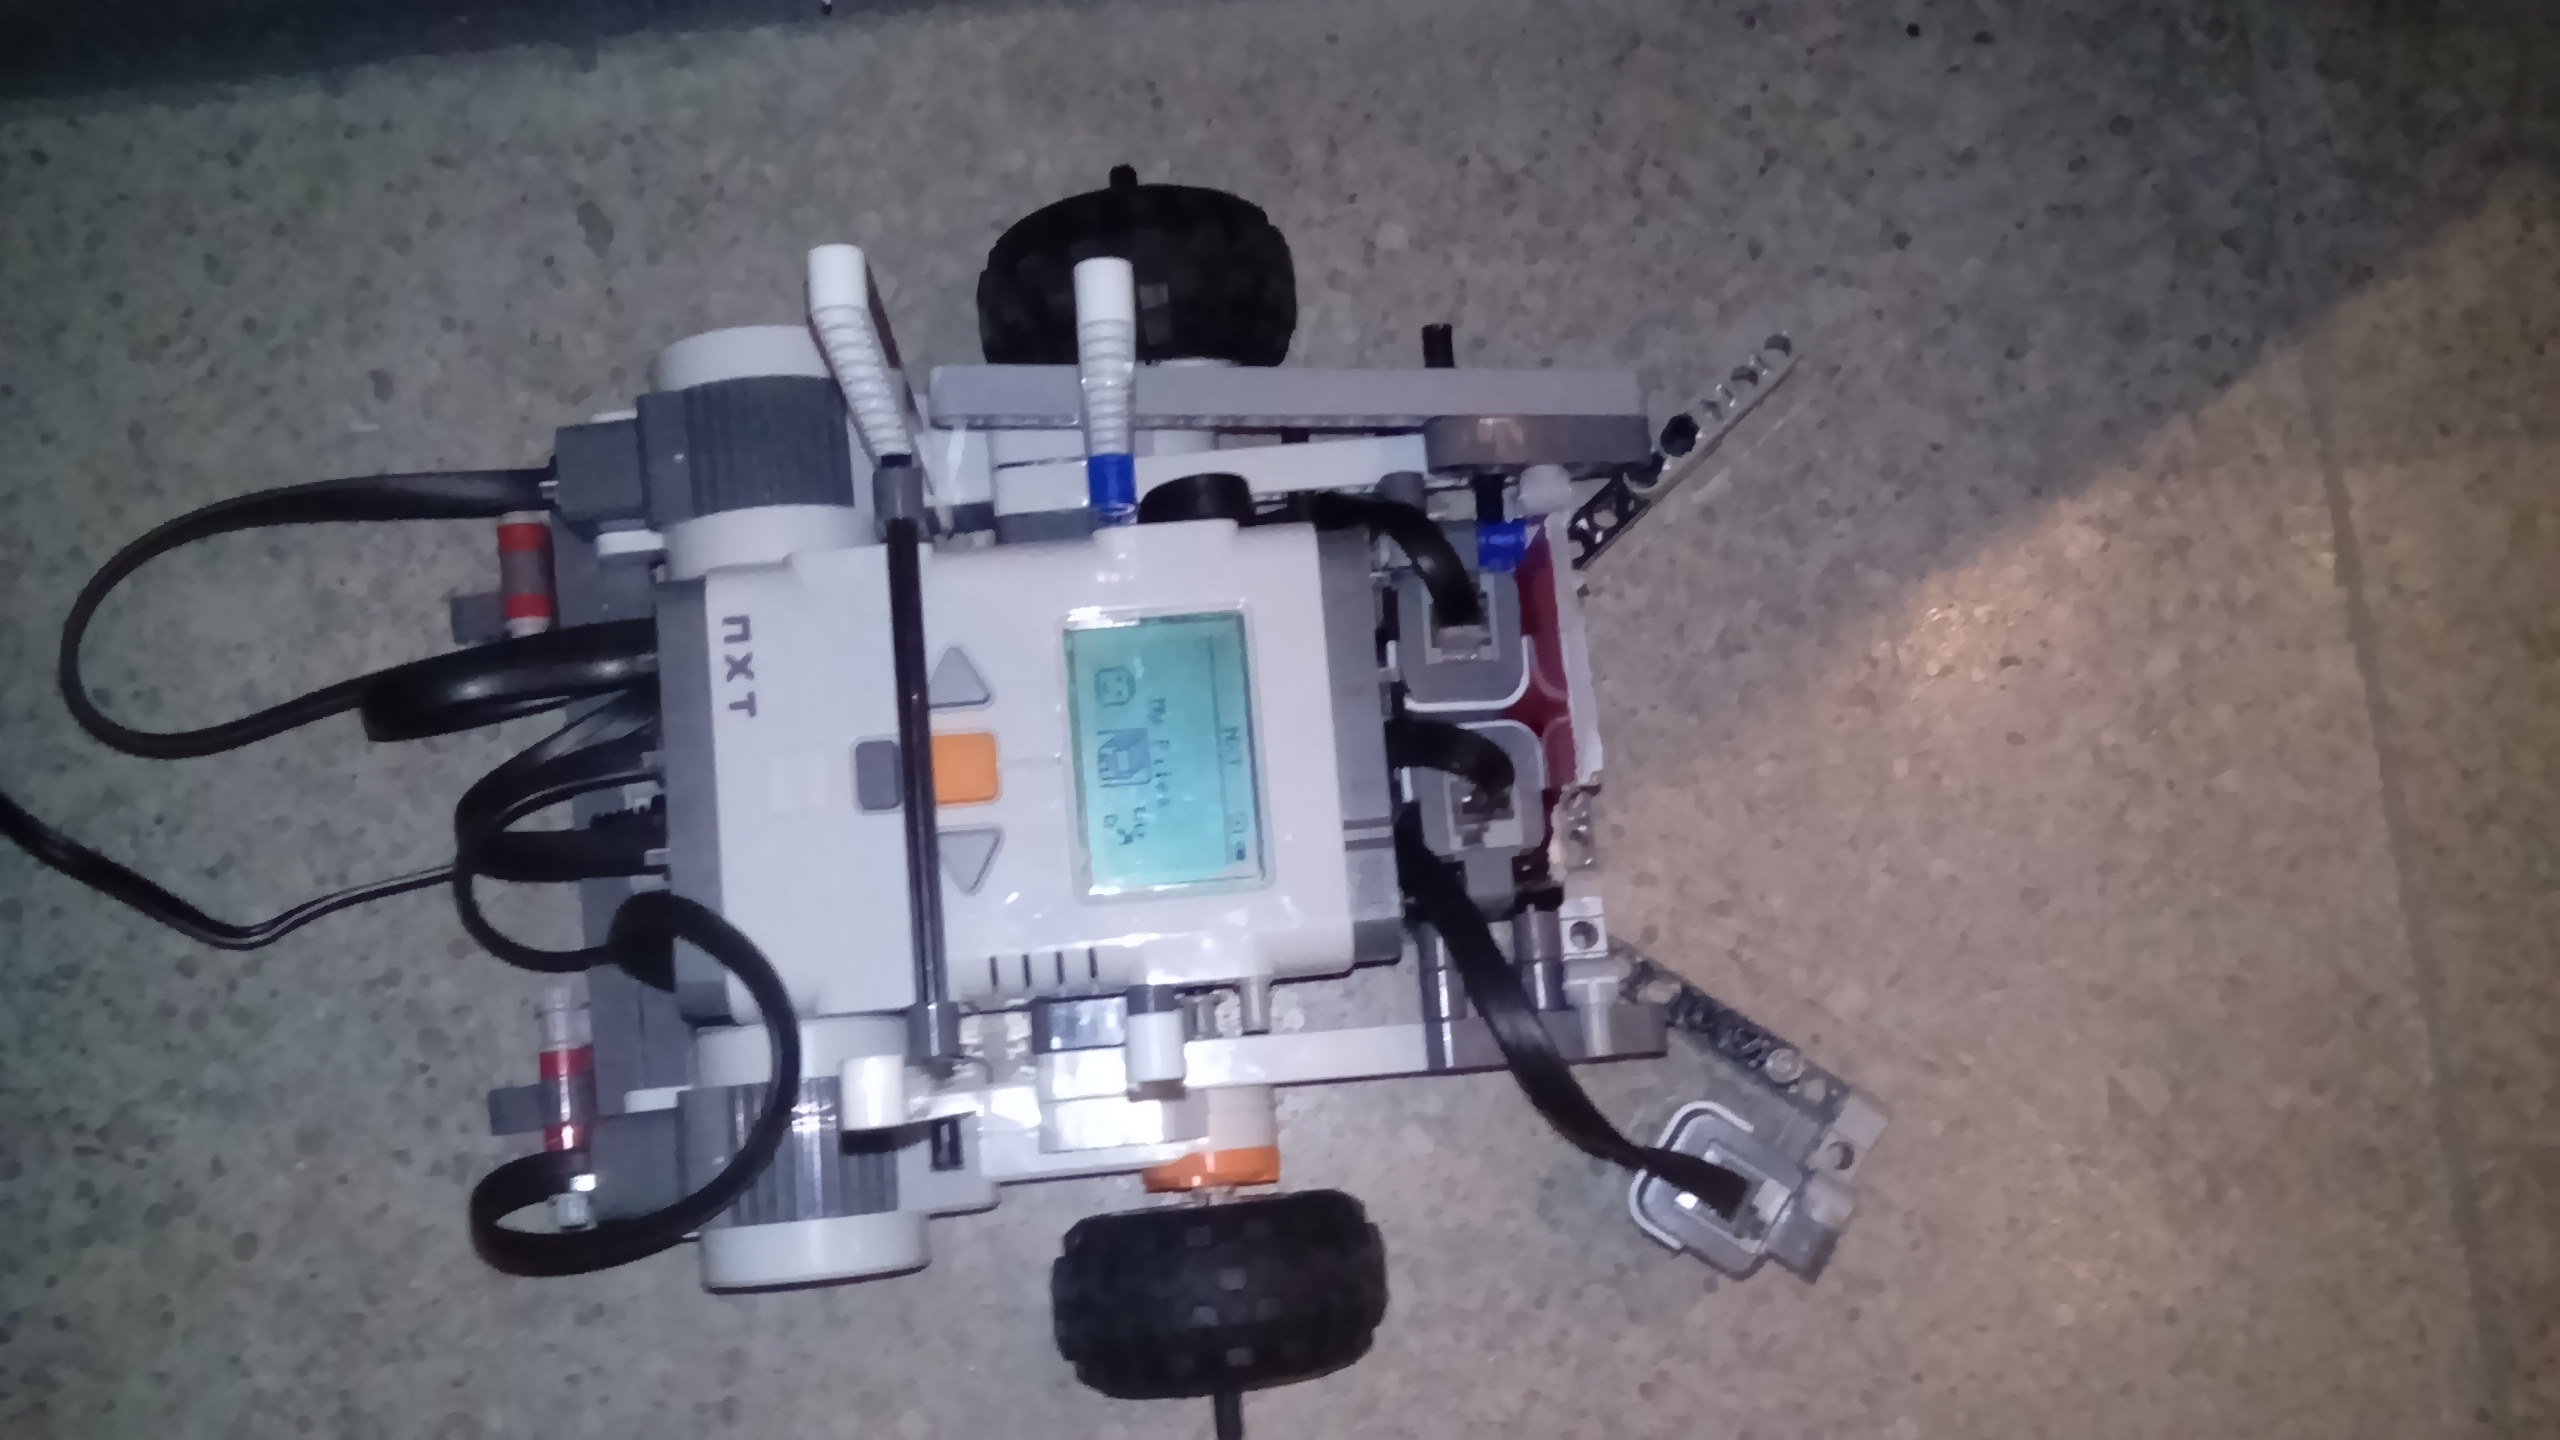
\includegraphics[scale = 0.1]{img/robot.jpg}
 \caption{Final design of the robot}
 \label{fig:final_robot}
\end{figure}

\subsubsection{Lego kit}

The lego kit used in this project contains a NXT brick and some sensors and actuators. A description of the sensors can be found in \cite{url:legosensors}. The number of different sensors and actuators in the kit can be seen in table \ref{tab:sensors}.

\begin{table} [H]
 \centering
 \begin{tabular}{|c|c|}
  \hline
  Sensor &  \# \\ \hline
  Light & 3 \\
  Touch & 2 \\
  Sound & 1 \\
  Ultrasound & 1 \\
  Motor & 3 \\
  \hline
 \end{tabular}
  \caption{Sensor types and the number of them in the kit}
  \label{tab:sensors}
\end{table}


\subsection{Sensing}\label{sec:sensing}
In order to sense the world around it, the robot was fitted with three light sensors. There were only three light sensors, so a decision had to be made on what to use the sensors for. All of the other types of sensors were deemed useless for this project.

The problems that needed to be addressed in the project was turning exactly $90^{\circ}$, stopping with the can on the intersection and line following.

It was quickly established that two sensors were needed for a line follow controller. The last sensor could then be used for a few things, e.g as indicator that a turn was completed or a detector of intersections. Both uses were tried and pros and cons were noted, and a decision was made on what was the best configuration. The two line following sensors were put as close together as it was possible with the chosen skeleton. It is worth noting that the distance between the sensors were bigger than the width of the line.

\begin{figure}[H]
 \begin{subfigure}{0.32\textwidth}
 \centering
    \begin{tikzpicture}

      \begin{scope}[rotate=-90]
	\draw node[robot_plain,rotate=-90] at (0,0) {};
      \end{scope}
    \end{tikzpicture}
  \caption{Plain robot configuration.}
  \label{subfig:plain_robot}
 \end{subfigure}
 %
 \begin{subfigure}{0.32\textwidth}
 \centering
    \begin{tikzpicture}

      \node[name=P_r] at (0.5,0) {};
      \begin{scope}[rotate=-90]
	\draw node[robot_back,rotate=-90] at (P_r) {};
      \end{scope}
    \end{tikzpicture}
  \caption{Rotational strong robot.}
  \label{subfig:rot_robot}
 \end{subfigure}
 %
 \begin{subfigure}{0.32\textwidth}
 \centering
    \begin{tikzpicture}
      \node[name=P_r] at (1,0) {};
      
      \begin{scope}[rotate=-90]
	\draw node[robot,rotate=-90] at (P_r) {};
      \end{scope}
    \end{tikzpicture}
  \caption{Final configuration.}
  \label{subfig:final_robot}
 \end{subfigure}
\caption{Illustration of the different configuration that was used during the project.}
\label{fig:line_follow}
\end{figure}

The first configuration, seen on figure \ref{subfig:plain_robot}, with no third sensor failed at turning properly, which led to the basis of the line following being poor. This made the line follow fail after a few turns. Putting a sensor on in the behind the center of the robot solved this problem. The placement can be seen in figure \ref{subfig:rot_robot}. 
With this setup, the pushing the can too far off an intersection became a problem.
This was giving the robot problems when having to move the same can from another direction as the can forced the robot off the line.
This could be solved by putting the third sensor on the gripper so that the center of the can is in line with the sensor, as seen in figure \ref{subfig:final_robot}. 
By doing this the can would always end on the intersection. 

It was assumed that the latter construction was the best, due to the severity of getting off the line in the line following, compared to having a bad starting point for it. Therefore this design was chosen as the final configuration.

\subsubsection{External Noise}
When using a light sensor the world around it can effect the value of the sensor tremendously.
A way to use the sensors is to just use a threshold value on the intensity to indicate that a line has been met.
This is not very robust as light intensity is difficult to control.
Assuming the sensor gives equal values on similar surfaces, lines can be detected by looking at the change of intensity.
This was implemented and was found to be stable.

\subsection{Sokoban Execution}

In order to execute the solution given by the solver, which is in game moves a translator needed to be implemented. This is due to the grid structure of the map, and a can push not being instantaneous in the real world.

The translator is implemented by looking at the current and previous game move. These are put into a look up table and the combination of robot moves found in the result from the look up is executed. 

\vspace{10pt}
{\large \textit{Example:}}

\noindent
Movestring ...\textbf{Luur}... (big characters are can pushes)

\noindent
Input to lookup: current = \textbf{u}, previous = \textbf{L}.

\noindent
Output from lookup: \textit{back, turn left, go forwards}

The next characters to be analyzed is then \textbf{uu}.
A lookup is then performed again, and the result is then:

\noindent
Input to lookup: current = \textbf{u}, previous = \textbf{u}.

\noindent
Output from lookup: \textit{go forwards}

The last sequence is \textbf{ur}. The lookup results in:

\noindent
Input to lookup: current = \textbf{r}, previous = \textbf{u}.

\noindent
Output from lookup: \textit{turn right, go forwards}

The lookup table it self is a \lstinline|switch case| that executes the commands one by one, in the correct order.